% TrustNav : article au format conférence IEEE (version française). Version anglaise : trustnav.tex
% Compilation :  cd paper && pdflatex trustnav_fr.tex && pdflatex trustnav_fr.tex
% Figures : python3 figures/make_figures.py (PDF vectoriels produits à partir des données d'évaluation)
\documentclass[conference]{IEEEtran}
\IEEEoverridecommandlockouts
\usepackage[utf8]{inputenc}
\usepackage[T1]{fontenc}
\usepackage[french]{babel}
\usepackage{cite}
\usepackage{amsmath,amssymb}
\usepackage{graphicx}
\usepackage{booktabs}
\usepackage{array}
\usepackage{xurl}
\usepackage{xcolor}
\usepackage{tikz}
\usetikzlibrary{arrows.meta,positioning}
\usepackage{balance}
\usepackage{dblfloatfix}
\usepackage[hidelinks]{hyperref}
\newcommand{\sys}{TrustNav}
\addto\captionsfrench{\renewcommand{\tablename}{Tableau}\renewcommand{\figurename}{Fig.}\renewcommand{\abstractname}{R\'esum\'e}}
\renewcommand{\IEEEkeywordsname}{Mots-cl\'es}
\frenchsetup{StandardItemLabels=true,StandardLists=true}

\begin{document}

\title{\sys\ : score de confiance explicable seconde par seconde et réponse au leurrage et au brouillage GNSS pour les flottes de véhicules et de drones}

\author{
\IEEEauthorblockN{Karan Deshmukh, Niranjan Satheesh Thandassery, Sudheer Reddy Jogi, Venkata Pavan Kumar Sanam}
\IEEEauthorblockA{MSc Cybersécurité et Science des données, ESAIP École d'Ingénieurs, Angers, France\\
Groupe 2, projet technique encadré par Sofiane Hamrioui\\
Auteur correspondant : domail2karandeshmukh@gmail.com}
}

\maketitle

\begin{abstract}
Les logiciels de flotte croient la position satellitaire que leurs récepteurs rapportent. Le brouillage et le leurrage sont désormais quotidiens dans certaines régions d'Europe et ne demandent qu'un matériel bon marché ; pourtant les contre-mesures existantes vivent soit dans un seul récepteur, qui émet un drapeau sans explication, soit dans une sonde fixe. Nous présentons \sys, une couche logicielle qui note chaque seconde, pour chaque véhicule et drone d'une flotte, à quel point sa position peut être crue (0--100), explique ce score en mots simples et \emph{répond} : une position sous le seuil de confiance est refusée et remplacée en aval par une estimation à l'estime, à partir de l'odomètre, le long de l'itinéraire prévu. Trois sortes de preuves sont fusionnées par un OU bruité : quinze règles à seuils nommés, un modèle d'anomalies non supervisé (forêt d'isolation et détecteur de queues) entraîné sur des trajets normaux seulement, et l'authentification Galileo OSNMA. Sur dix scénarios de test issus d'un simulateur déterministe sur les rues réelles d'Angers (3\,800 observations d'une seconde), le détecteur combiné atteint 99,3\,\% de précision, 96,1\,\% de rappel et 0,44\,\% de fausses alertes, détecte les sept types d'attaque et repère en 42\,s une dérive « furtive » qui passe l'OSNMA, là où une règle fixe à 150\,m aurait besoin d'environ 3,5\,min. La couche de réponse ramène la pire erreur visible par l'opérateur de 8,0\,km à 29\,m et supprime l'écran vide de 100\,s causé par le brouillage. Le système est en source ouverte ; ses limites (données entièrement synthétiques) et le plan de validation sur un récepteur réel sont discutés.
\end{abstract}

\begin{IEEEkeywords}
GNSS, leurrage, brouillage, Galileo OSNMA, détection d'anomalies, forêt d'isolation, IA explicable, télématique de flotte, navigation à l'estime, cybersécurité.
\end{IEEEkeywords}

\section{Introduction}
Presque tout ce qui se déplace, des camionnettes de livraison aux navires et aux drones, s'appuie sur une position GNSS (système mondial de navigation par satellite) et lui fait confiance sans la remettre en question. Cette confiance est facile à briser : les signaux GNSS, émis à 20\,000\,km, sont extrêmement faibles au sol, et un petit émetteur proche peut les noyer (\emph{brouillage}) ou les imiter et fournir au récepteur une position fausse mais plausible (\emph{leurrage}). Des brouilleurs à quelques dizaines d'euros sont vendus illégalement et régulièrement trouvés dans des véhicules dont le conducteur veut échapper au suivi de sa flotte \cite{anfr2024} ; l'un d'eux, laissé allumé dans une voiture garée à l'aéroport de Nantes, a retardé des vols en 2017 \cite{rntf2017}, un autre a perturbé une aide à l'atterrissage de l'aéroport de Lyon en 2023 \cite{transinfo2023}. Depuis 2022, les interférences autour de la Baltique et au Moyen-Orient sont quotidiennes pour l'aviation : environ 1\,500 vols leurrés par jour à l'été 2024 \cite{eucouncil2025,opsgroup2024}.

Deux lacunes motivent ce travail. D'abord, les plateformes télématiques des exploitants affichent la position rapportée et, au mieux, relaient le drapeau de brouillage du récepteur \cite{geotab2025} ; elles ne disent pas si la position est vraie. Ensuite, les produits de détection existants tournent soit dans un récepteur, avec un code d'état sans explication \cite{ublox2024,septentrio2025}, soit dans des sondes fixes multi-antennes qui protègent un site et non une plateforme mobile \cite{gpspatron}. La place naturelle d'une défense est selon nous une couche logicielle à côté du récepteur, travaillant sur ce que tout récepteur rapporte déjà, qui (i) donne à chaque plateforme un score de confiance par seconde, (ii) l'explique en termes vérifiables par un opérateur et (iii) agit pour que rien en aval ne consomme un mensonge. \sys\ est cette couche. Nos contributions :
\begin{enumerate}
\item un détecteur hybride qui fusionne quinze règles explicables, un modèle d'anomalies non supervisé entraîné sur le seul fonctionnement normal et l'état OSNMA de Galileo, avec une conversion calibrée de la probabilité d'anomalie en risque qui donne au seuil d'alerte un sens énoncé ;
\item une \emph{couche de réponse} qui refuse les positions non fiables et leur substitue une estimation à l'estime sur l'itinéraire, à partir de l'odomètre, avec une règle de reprise qu'un leurreur ne peut pas contourner en paraissant brièvement propre ;
\item une implémentation complète et ouverte : moteur Python, serveur en nuage, console qui explique chaque décision en mots simples, adaptateur pour récepteurs réels ;
\item un protocole d'évaluation à itinéraires d'entraînement, de validation et de test disjoints sur les rues réelles d'Angers, et une mesure chiffrée de ce que la couche de réponse évite.
\end{enumerate}

\section{Contexte et travaux connexes}\label{sec:related}

\subsection{Menaces}
Un \emph{brouilleur} émet du bruit dans les bandes GNSS : le rapport porteuse sur bruit (C/N$_0$) s'effondre, les satellites sont perdus et plus aucune position n'est calculée. Un \emph{leurreur} émet de faux signaux satellitaires ; un leurreur simple capture le récepteur et déplace la position d'un coup (« téléportation »), un leurreur prudent l'éloigne lentement (« dérive »). Une attaque par \emph{relais} (\emph{meaconing}) rediffuse des signaux authentiques avec un retard : les données de navigation restent authentiques, la position est fausse. La \emph{falsification} fabrique les messages de navigation eux-mêmes. Chacune laisse des traces différentes dans les observables du récepteur : mouvement impossible, signaux trop forts et trop uniformes, résidus discordants, sauts d'horloge ou échec d'authentification.

\subsection{Galileo OSNMA}
L'authentification des messages de navigation du service ouvert de Galileo signe les données I/NAV par un schéma TESLA à divulgation différée ; elle est opérationnelle depuis le 24 juillet 2025 \cite{euspa2025} et obligatoire dans les tachygraphes intelligents des nouveaux poids lourds de l'UE dès décembre 2025. Elle permet de signaler des données non authentifiées, mais le Centre de services GNSS européen précise qu'elle ne protège pas du brouillage et n'empêche pas à elle seule le leurrage \cite{gsc_faq} ; le GPS n'est pas couvert, et des attaques par rejeu qui passent l'OSNMA ont été démontrées sur des récepteurs réels \cite{wang2025}. L'OSNMA est une preuve parmi d'autres, pas une défense complète.

\subsection{Contre-mesures existantes}
Les récepteurs grand public u-blox rapportent un état de leurrage (inconnu, aucun, indiqué, indications multiples) et un état de brouillage ; les micrologiciels récents ajoutent un journal de brouillage, l'OSNMA et des drapeaux par bande \cite{ublox2024}. Le fabricant précise qu'un état « pas de leurrage » ne prouve rien, et au Jammertest 2025 les deux drapeaux se sont déclenchés lors d'un essai de brouillage seul \cite{ublox_jammertest}. Septentrio intègre de même filtres, vue spectrale et drapeaux de leurrage dans ses récepteurs \cite{septentrio2025}. Les sondes de GPSPatron (jusqu'à trois antennes espacées d'au moins 1\,m) envoient leurs observables bruts à un nuage qui classe les attaques \cite{gpspatron} ; le GPSdome d'infiniDome annule les brouilleurs avec deux antennes ou plus \cite{gpsdome2}. Les boîtiers GO récents de Geotab journalisent un événement de brouillage levé par le module GPS \cite{geotab2025} ; aucun fournisseur télématique examiné ne revendique de détection du leurrage. Le tableau~\ref{tab:compare} résume ces différences ; \sys\ consomme les drapeaux des récepteurs et l'OSNMA comme entrées plutôt que de les concurrencer.

\begin{table*}[t]
\caption{Ce qui distingue \sys\ de l'existant (sources en section~\ref{sec:related})}
\label{tab:compare}
\centering
\scriptsize
\setlength{\tabcolsep}{4pt}
\begin{tabular}{@{}>{\raggedright}p{2.2cm}>{\raggedright}p{2.15cm}>{\raggedright}p{2.15cm}>{\raggedright}p{2.15cm}>{\raggedright}p{2.15cm}>{\raggedright}p{2.15cm}>{\raggedright\arraybackslash}p{2.9cm}@{}}
\toprule
 & Drapeaux du récepteur (u-blox, Septentrio) & Sondes fixes (GPSPatron) & Matériel anti-brouillage (infiniDome) & Télématique de flotte (Geotab, etc.) & OSNMA & \textbf{\sys} \\
\midrule
Protège & un récepteur & un site ou une région & un récepteur & l'écran de flotte & les données Galileo & \textbf{chaque plateforme mobile} \\
Détecte & brouillage, leurrage & brouillage, leurrage & brouillage (atténue) & relaie le drapeau de brouillage du récepteur & données Galileo falsifiées & \textbf{brouillage, leurrage, falsification} \\
Score par seconde & non (code d'état) & probabilité & non & non & non & \textbf{oui, 0--100} \\
Explique pourquoi & non & en partie (courbes) & non & non & s.o. & \textbf{oui, en mots avec les valeurs} \\
Itinéraire, odomètre & non & non & non & non & non & \textbf{oui} \\
Répond & non & alertes & oui (annulation RF) & rapport & drapeau & \textbf{refuse la position, estime, recommande une action} \\
Matériel en plus & aucun & sonde, 1 à 3 antennes & 2 antennes ou plus & aucun & récepteur compatible OSNMA & \textbf{aucun} \\
\bottomrule
\end{tabular}
\end{table*}

\subsection{Détection par apprentissage automatique}
Des travaux récents appliquent des modèles appris aux observables du récepteur, surtout sur les enregistrements TEXBAT \cite{texbat} : un réseau LSTM avec VAE conditionnel atteint un F$_1$ de 96,9\,\% \cite{tang2025} ; un VAE convolutif entraîné sur données propres seulement atteint des taux de vrais positifs presque parfaits sur les jeux faciles et 89\,\% sur le plus difficile \cite{iqbal2025} ; une forêt aléatoire dépasse 97\,\% \cite{li2025} ; un test du khi-deux sur les échantillons bruts en fréquence intermédiaire rapporte plus de 99\,\% d'exactitude sans fausse alerte \cite{bhuiyan2026}. Au plus près de notre cadre, Kriezis \emph{et al.} ont évalué des règles sur un u-blox ZED-F9P à 200\,\texteuro\ face à du leurrage réel en Méditerranée orientale : C/N$_0$, résidus et dérive d'horloge étaient informatifs, le contrôle de gain et le Doppler non, et l'algorithme d'interférence des MOPS aéronautiques obtenait 94\,\% sur un récepteur mais moins de 13\,\% sur un autre \cite{kriezis2025}. \sys\ appartient à la même famille mais est un \emph{système} : il ajoute l'itinéraire et l'odomètre, preuves qu'un récepteur ne peut pas fournir, rapporte une confiance par seconde plutôt qu'un verdict binaire, explique chaque décision et répond.

\section{Conception du système}\label{sec:design}

\begin{figure}[t]
\centering
\begin{tikzpicture}[font=\scriptsize, x=1cm, y=1cm,
  box/.style={draw, rounded corners=1.5pt, align=center, inner sep=2pt, minimum height=7.5mm, text width=1.55cm},
  sink/.style={box, fill=black!6},
  arr/.style={-{Latex[length=1.6mm]}, thick}]
\node[box] (obs) at (0,0) {Observation du\\récepteur (1 Hz)};
\node[box] (feat) at (2.25,0) {36 caractéristiques\\(fenêtre 5 s, itinéraire)};
\node[box] (rules) at (4.5,0.65) {15 règles\\(OU bruité)};
\node[box] (model) at (4.5,-0.65) {Modèle d'anomalies\\(IF + queues)};
\node[box] (fuse) at (6.75,0) {Fusion\\confiance $=100-$risque};
\node[box] (resp) at (6.75,-1.95) {Réponse\\accepter / maintenir};
\node[sink] (down) at (4.5,-1.95) {Logiciels\\en aval};
\node[sink] (inc) at (2.25,-1.95) {Incidents, console,\\nuage};
\draw[arr] (obs) -- (feat);
\draw[arr] (feat) -- (rules);
\draw[arr] (feat) -- (model);
\draw[arr] (rules) -- (fuse);
\draw[arr] (model) -- (fuse);
\draw[arr] (fuse) -- (resp);
\draw[arr] (resp) -- (down);
\draw[arr] (resp.south) -- ++(0,-0.3) -| (inc.south);
\end{tikzpicture}
\caption{Chaîne de traitement. Chaque observation (position, vitesse, signal, horloge, état OSNMA, vitesse odométrique) devient un vecteur de caractéristiques, est jugée par les règles et par un modèle d'anomalies, fusionnée en un score de confiance avec ses preuves, puis transmise à la couche de réponse, qui décide quelle position les logiciels en aval reçoivent.}
\label{fig:pipeline}
\end{figure}

\subsection{Observations et caractéristiques}
Chaque seconde, le récepteur rapporte position, vitesse, cap, satellites suivis, statistiques de C/N$_0$, dilution de précision (PDOP), résidus de pseudo-distance, biais et dérive d'horloge, un indicateur de brouillage, l'état OSNMA et, lorsqu'elle existe, une vitesse inertielle ou odométrique (fig.~\ref{fig:pipeline}). Ce qui compte est la comparaison d'une lecture avec les secondes précédentes et avec l'itinéraire prévu ; un extracteur en flux conserve donc une fenêtre glissante de cinq observations et calcule 36 caractéristiques : distance parcourue, vitesse dérivée contre vitesse rapportée, accélération et rotation du cap, distance à l'itinéraire, moyenne, variation et dispersion du C/N$_0$, variation du nombre de satellites, PDOP, résidus, écarts d'horloge, désaccord entre vitesse GNSS et vitesse inertielle, et des drapeaux \texttt{missing\_*} pour qu'une entrée absente ne passe jamais pour un zéro. L'extracteur est incrémental : le même code note l'enregistré et le direct.

\subsection{Règles}
Quinze vérifications déterministes comparent une caractéristique à un seuil nommé, tiré du profil physique de la plateforme (véhicule routier : 60\,m/s, 8\,m/s$^2$, 90$^\circ$/s, 250\,m par seconde) ou de la physique du signal (décalage de C/N$_0$ de 6\,dB-Hz, PDOP au-dessus de 5, résidus au-dessus de 12\,m, variation de dérive d'horloge au-dessus de 60\,ns/s, indicateur de brouillage au-dessus de 80/255, variation d'au moins cinq satellites), plus l'échec ou la perte de l'OSNMA et la perte de position. La contribution $c_i$ d'une règle est son poids multiplié par une sévérité qui monte de 0,5 au seuil à 1,0 à trois fois le seuil ; les règles se combinent par un OU bruité,
\begin{equation}
r_{\mathrm{r\grave{e}gles}} = 100\,\Bigl(1-\prod\nolimits_i (1-c_i)\Bigr),
\end{equation}
de sorte que des preuves indépendantes se renforcent. Deux conditions sont \emph{critiques} : un saut de position supérieur à quatre fois la limite du profil et un échec OSNMA ; chacune fixe le risque combiné à 70 au moins. Les seuils sont placés là où le comportement devient physiquement invraisemblable : les règles restent presque muettes sur les données normales, au prix des attaques lentes.

\begin{figure*}[t]
\centering
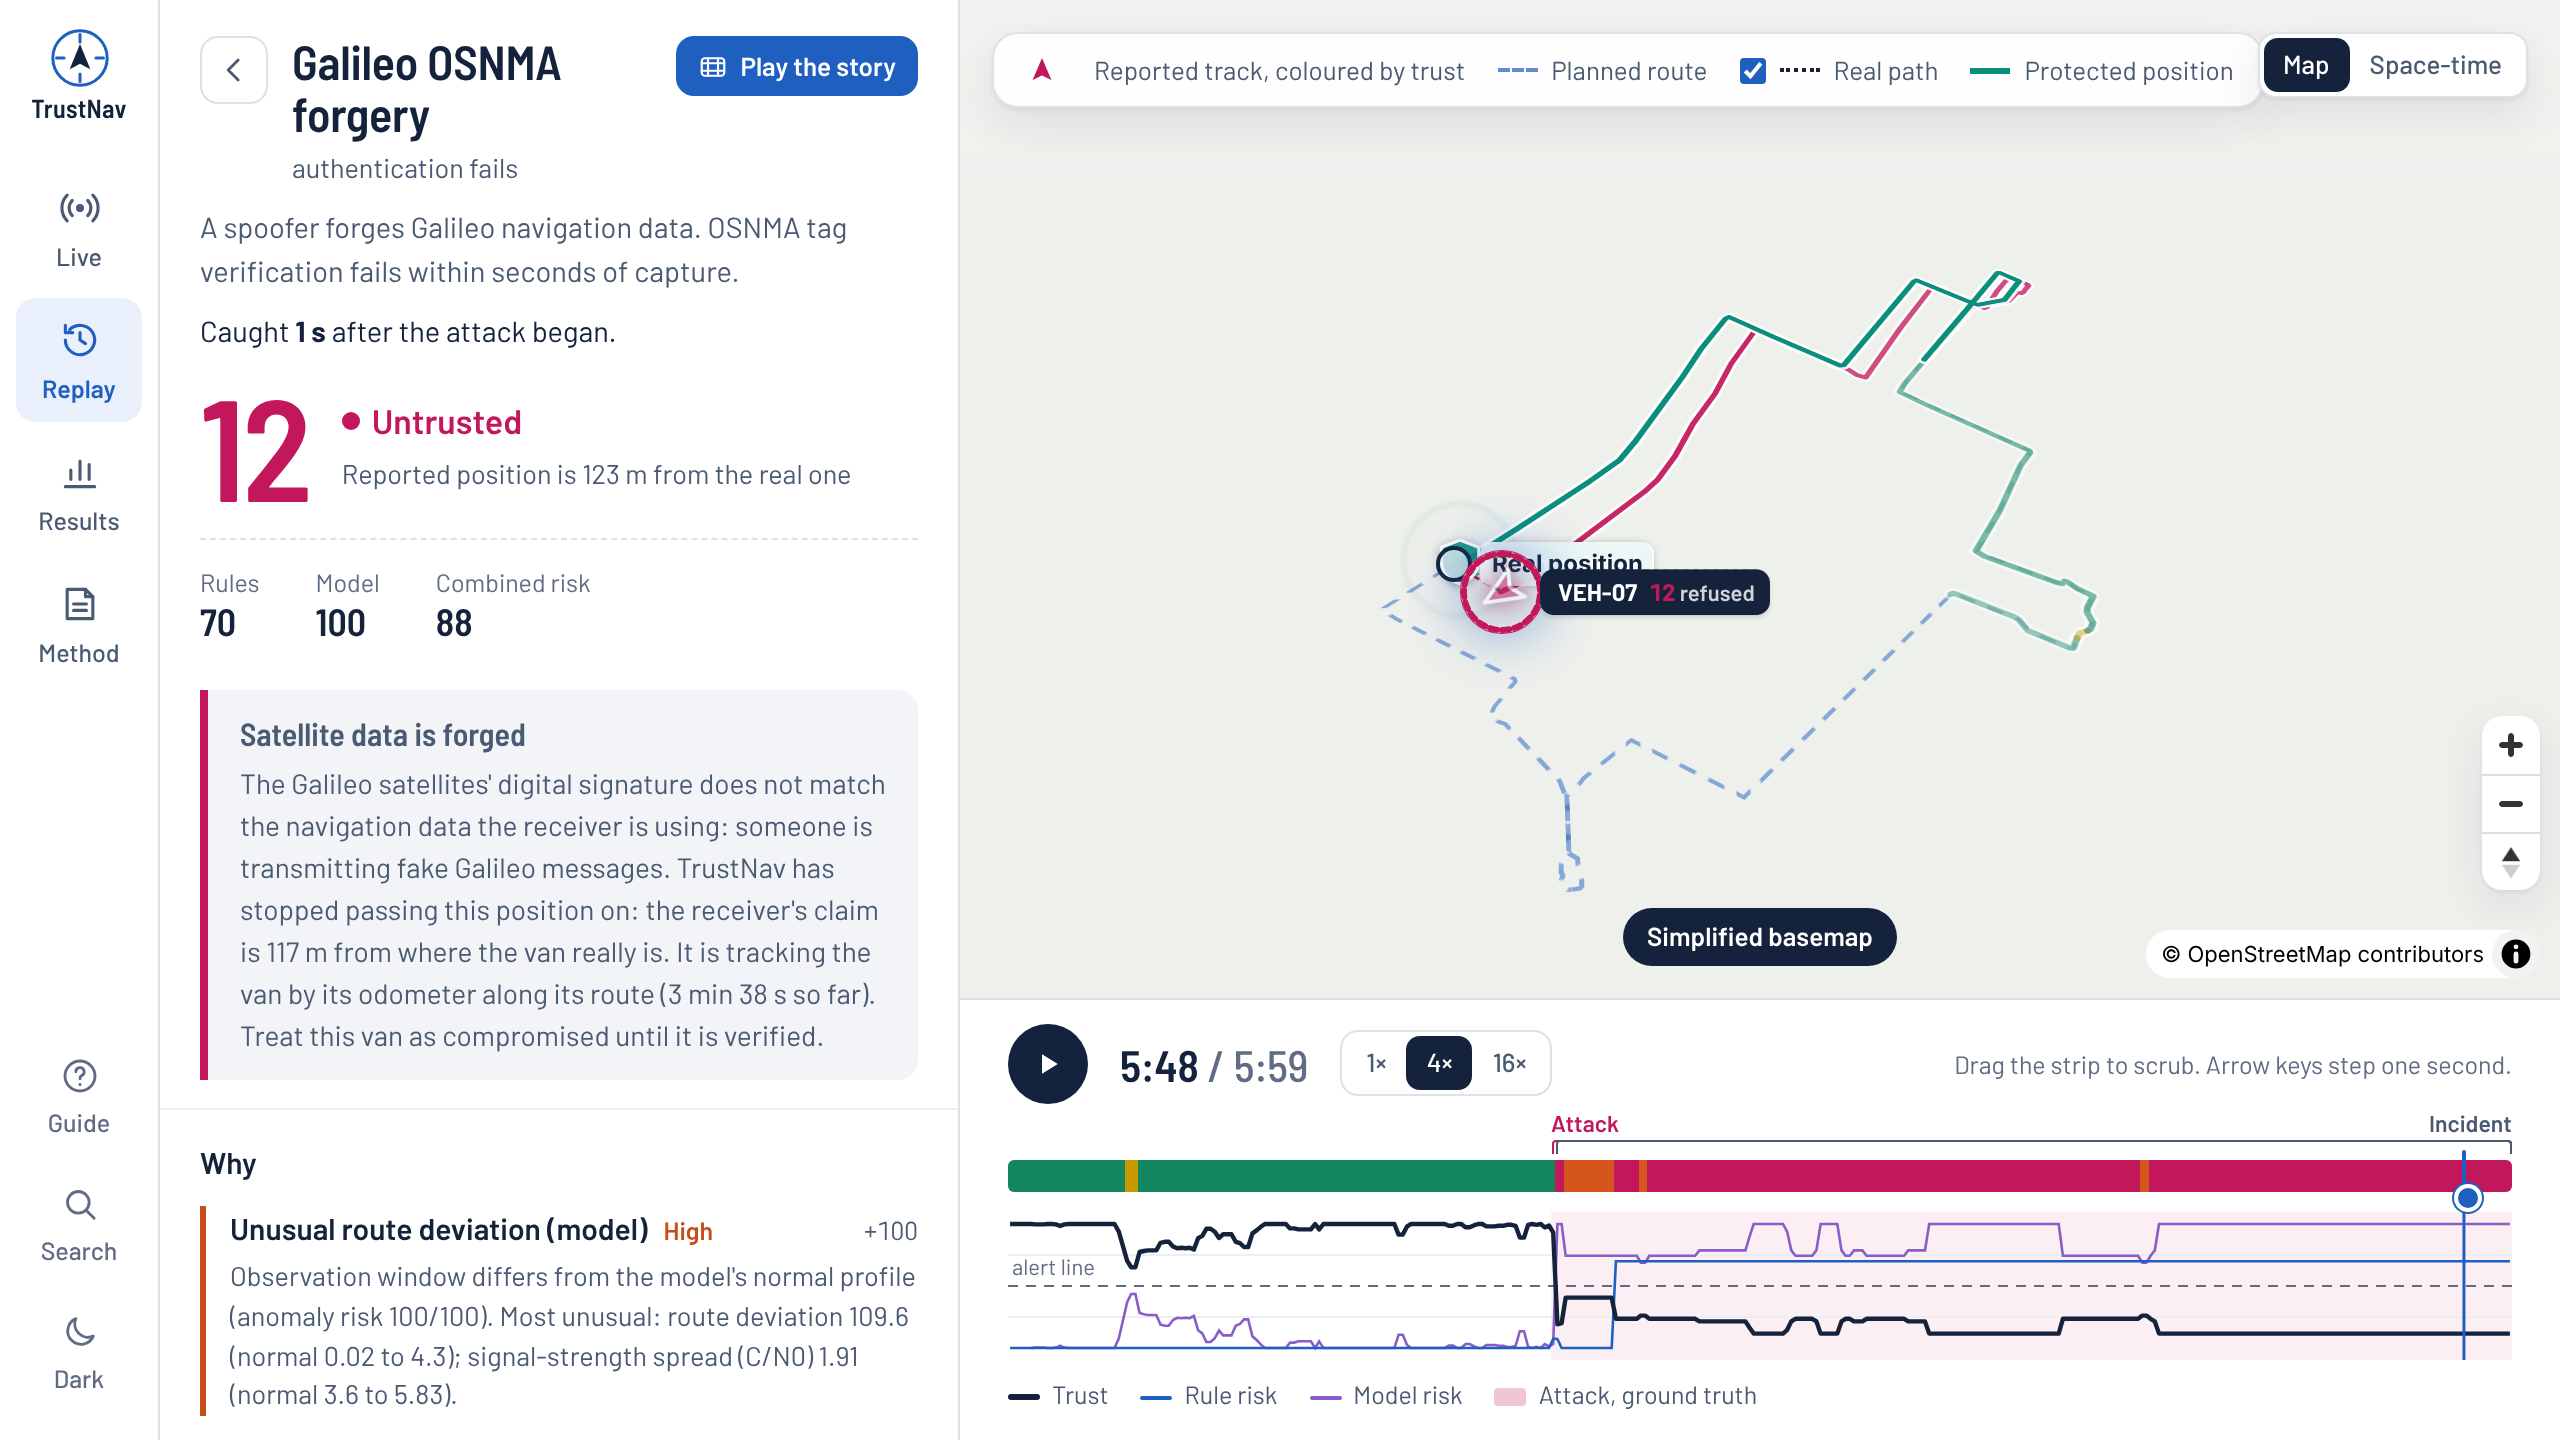
\includegraphics[width=0.68\textwidth]{figures/console-replay.png}
\caption{La console rejouant le scénario de falsification OSNMA (interface en anglais) : score et bande de confiance, les trois risques, le verdict en langage courant et les preuves avec valeurs et plages normales (à gauche) ; trace rapportée colorée par la confiance, itinéraire prévu, trajet réel et position protégée, position refusée marquée « 12 refused » (carte) ; courbes de confiance et de risque avec la fenêtre d'attaque et l'incident (en bas).}
\label{fig:console}
\end{figure*}

\subsection{Modèle d'anomalies}
Comme tout modèle supervisé apprendrait la forme des attaques du simulateur, la composante apprise est entraînée \emph{uniquement sur le fonctionnement normal}. Deux détecteurs se complètent : une forêt d'isolation \cite{liu2008} (300 arbres, scikit-learn \cite{sklearn}) trouve les combinaisons inhabituelles des 19 entrées du modèle, et un détecteur de queues par caractéristique trouve une seule entrée improbable, par exemple une position à 90\,m de la route alors que tout le signal est propre, et la nomme. Le score brut de chaque détecteur est converti en probabilité de queue $p$ sur des trajets normaux de calibration non utilisés pour l'ajustement (fraction d'observations normales au moins aussi anormales), les deux sont combinés avec une correction de Bonferroni, $p=\min(1,\,2\min(p_{\mathrm{for\hat{e}t}},p_{\mathrm{queue}}))$, et le risque vaut
\begin{equation}
r_{\mathrm{mod\grave{e}le}} = 100\,\min\!\left(1,\ \frac{-\log_{10} p}{4}\right),
\end{equation}
de sorte qu'un risque de 50 correspond à peu près à un événement sur cent en fonctionnement normal, alors qu'un simple rang centile déclencherait une alerte à 50 sur la moitié des secondes propres. Une médiane glissante sur trois secondes supprime les pics isolés. À partir d'un risque de 25, le modèle s'explique en listant ses entrées les plus inhabituelles avec leurs plages normales.

\subsection{Fusion, confiance et incidents}
Règles et modèle sont deux témoins, pas deux votes à moyenner : une alarme du modèle à 90 moyennée avec des règles silencieuses à 20 donnerait 55, moins que le modèle seul. Le risque combiné est un OU bruité pondéré,
\begin{equation}
r = 100\,\bigl(1-(1-w_r\,p_r)(1-w_m\,p_m)\bigr),
\end{equation}
avec $p_r=r_{\mathrm{r\grave{e}gles}}/100$ et $p_m=r_{\mathrm{mod\grave{e}le}}/100$, et la confiance vaut $100-r$. Les poids $w_r=0,6$ et $w_m=0,8$ ont été choisis par recherche en grille sur les seuls itinéraires de validation. Les bandes de confiance sont Fiable ($\ge75$), Dégradée (50--74), Suspecte (25--49) et Non fiable ($<25$). Un incident s'ouvre après trois secondes consécutives sous 50 et se ferme après cinq secondes propres ; son titre nomme la preuve critique la plus forte.

\subsection{Couche de réponse}
La détection seule laisse l'opérateur face à un mensonge. La couche de réponse transforme le score en action, comme un système de \emph{prévention} d'intrusion agit sur ce qu'un système de \emph{détection} trouve. Une position est \emph{acceptée} quand elle existe, que sa confiance est d'au moins 50 et qu'aucune règle critique ne s'est déclenchée. Sinon elle est \emph{maintenue} : la position est refusée et celle transmise en aval est calculée à l'estime depuis la dernière position acceptée, avec la vitesse odométrique, qu'un leurreur ne peut pas toucher. Avec un itinéraire assigné, l'estimation avance le long de l'itinéraire (appariement cartographique) : l'erreur latérale de la dernière position acceptée disparaît et seule l'erreur odométrique s'accumule ; sans itinéraire, elle continue sur le dernier cap accepté. Un maintien n'est \emph{levé} qu'après cinq observations acceptables consécutives dont la position est à moins de 60\,m plus 3\,\% de la distance parcourue à l'estime, pour qu'un leurreur ne puisse pas y mettre fin en paraissant propre tout en restant loin ; soixante secondes propres le lèvent quoi qu'il arrive, en signalant l'écart, car une estimation odométrique dérive aussi. Chaque observation porte une action recommandée : \textsc{continuer}, \textsc{vérifier} (confirmer par un autre moyen avant d'agir) ou \textsc{isoler} (confiance sous 25 ou preuve critique : cesser d'utiliser la position, rappeler le drone en inertiel, contacter le conducteur).

\section{Implémentation}\label{sec:impl}
\sys\ est en source ouverte\footnote{\url{https://github.com/domail2karandeshmukh-cyber/trustnav}} et déployé comme démonstration publique\footnote{\url{https://trustnav.vercel.app}}. Le \textbf{moteur} est en Python (NumPy, scikit-learn) : simulateur déterministe, extracteur de caractéristiques, règles, modèle, fusion, suivi des incidents, couche de réponse, évaluation et diffuseur en direct, avec 23 tests automatisés. Un \textbf{adaptateur de récepteur} convertit les trames NMEA (GGA, RMC, VTG, GSA, GSV) et les messages UBX u-blox (NAV-PVT, NAV-CLOCK, NAV-STATUS, NAV-SAT, MON-HW), depuis un port série ou un journal, vers le même dictionnaire d'observation : un récepteur réel se branche sur le même détecteur. Le côté \textbf{nuage} est Supabase (PostgreSQL avec sécurité par ligne, canaux temps réel, flux de démonstration planifié) : le navigateur ne peut que lire, les écritures passent par une fonction qui vérifie un jeton stocké en condensé SHA-256, et aucun secret n'est dans le dépôt. La \textbf{console} (fig.~\ref{fig:console}) est une application Next.js avec une carte MapLibre d'Angers, une vue de flotte en direct, le rejeu des dix scénarios, une vue espace--temps et un explicatif narré en dix langues ; 98 vérifications de bout en bout s'exécutent à chaque construction. Chaque décision est expliquée deux fois : par les lignes de preuve du moteur (« Position déplacée de 8\,003\,m en 1\,s (limite 250\,m) ») et par un verdict en mots de tous les jours dérivé des seuls codes de preuve, donc valable tel quel sur un récepteur réel.

\begin{figure*}[t]
\centering
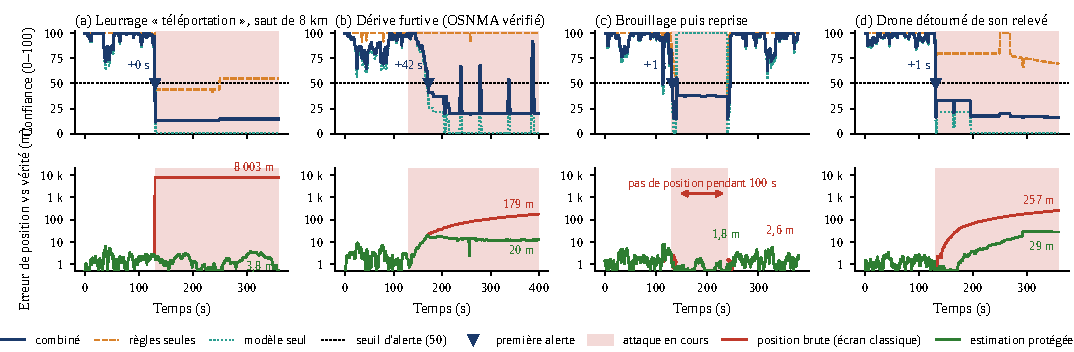
\includegraphics[width=0.9\textwidth]{figures/fig_timeline_fr.pdf}
\caption{Quatre scénarios de test, seconde par seconde. En haut : confiance du détecteur combiné et de chaque témoin seul ; le marqueur est la première alerte, avec son délai après le début de l'attaque. En bas : erreur de position par rapport à la vérité terrain pour la position brute qu'un écran ordinaire afficherait et pour l'estimation transmise en aval (échelle logarithmique, maxima pendant l'attaque indiqués). En (b), aucune règle ne se déclenche et l'OSNMA vérifie toujours ; le modèle seul détecte la dérive.}
\label{fig:timeline}
\end{figure*}

\section{Évaluation}\label{sec:eval}

\subsection{Données et protocole}
Aucun jeu de données public ne fournit des observables de récepteur étiquetés par seconde pour des flottes avec itinéraires et odomètres, et émettre des attaques est illégal ; un simulateur déterministe à graine fixée produit donc les observations qu'un récepteur rapporterait. Les itinéraires routiers sont les rues réelles d'Angers, calculés avec OSRM sur OpenStreetMap ; les missions de drone sont des relevés en lacets. Le comportement normal inclut arrêts, virages et canyons urbains, sources habituelles de fausses alertes. Les attaques superposées, étiquetées par observation, sont : une téléportation de 8\,km par un leurreur GPS seul (l'OSNMA devient indisponible) ; une dérive progressive sous 1\,m/s, la puissance du leurreur restant visible dans le C/N$_0$ ; un début de leurrage où le C/N$_0$ saute et devient anormalement uniforme alors que la position bouge à peine ; une \emph{dérive furtive} de type relais, signal propre et OSNMA toujours vérifié ; une falsification OSNMA ; un brouillage large bande avec perte puis reprise de la position ; et un drone poussé hors de sa ligne de relevé.

Chaque itinéraire reçoit un seul rôle : cinq boucles routières et deux zones de drone pour l'\emph{entraînement} (trajets normaux seulement, 10\,785 observations pour l'ajustement et 5\,630 pour la calibration), deux boucles et une zone pour la \emph{validation} (poids de fusion seulement), et deux boucles et une zone pour le catalogue de \emph{test} qui produit chaque chiffre rapporté : dix scénarios, 3\,800 observations d'une seconde, dont 1\,550 sous attaque. L'unité d'évaluation est l'observation ; une alerte est un risque combiné d'au moins 50.

\subsection{Détection}
Le tableau~\ref{tab:detect} compare les trois façons de décider. Les règles ne lèvent jamais de fausse alerte mais manquent les attaques lentes ; le modèle capte les changements subtils mais est plus bruyant ; combinés, chacun couvre l'angle mort de l'autre. Le tableau~\ref{tab:scen} donne, par scénario, le délai entre le début de l'attaque et la première alerte, et la fig.~\ref{fig:timeline} montre quatre essais seconde par seconde. Les sept types d'attaque sont détectés ; la dérive furtive, invisible pour toutes les règles et pour l'OSNMA, est détectée par le modèle après 42\,s, à environ 12\,m de la route, là où la règle fixe à 150\,m aurait besoin d'environ 3,5\,min. La confiance remonte brièvement aux pauses de la dérive (fig.~\ref{fig:timeline}b) sans lever le maintien : la position reste loin de l'estimation.

\begin{table}[t]
\caption{Détection sur le catalogue de test (3\,800 observations)}
\label{tab:detect}
\centering
\footnotesize
\begin{tabular}{@{}lrrr@{}}
\toprule
 & Règles seules & Modèle seul & \textbf{Combiné} \\
\midrule
Précision & 100,0\,\% & 97,9\,\% & \textbf{99,3\,\%} \\
Rappel & 27,9\,\% & 90,1\,\% & \textbf{96,1\,\%} \\
F$_1$ & 0,437 & 0,939 & \textbf{0,977} \\
Taux de fausses alertes & 0,00\,\% & 1,33\,\% & \textbf{0,44\,\%} \\
AUC ROC & 0,857 & 0,937 & \textbf{0,990} \\
AUC précision--rappel & 0,832 & 0,951 & \textbf{0,990} \\
Délai moyen de détection & 9,0\,s & 6,6\,s & \textbf{6,7\,s} \\
\midrule
Vrais positifs & 433 & 1\,397 & 1\,489 \\
Faux positifs & 0 & 30 & 10 \\
Faux négatifs & 1\,117 & 153 & 61 \\
Vrais négatifs & 2\,250 & 2\,220 & 2\,240 \\
\bottomrule
\end{tabular}
\end{table}

\begin{table}[t]
\caption{Délai entre le début de l'attaque et la première alerte}
\label{tab:scen}
\centering
\footnotesize
\begin{tabular}{@{}lrrrr@{}}
\toprule
Scénario & Règles & Modèle & \textbf{Comb.} & FA \\
\midrule
Trajet normal, centre (420 obs.) & -- & -- & -- & 0 \\
Trajet normal, est (420) & -- & -- & -- & 2 \\
Téléportation, saut de 8\,km & 0\,s & 1\,s & \textbf{0\,s} & 0 \\
Dérive progressive & manqué & 1\,s & \textbf{1\,s} & 0 \\
Anomalie de signal (leurreur) & manqué & 1\,s & \textbf{1\,s} & 0 \\
Dérive furtive (OSNMA vérifié) & manqué & 40\,s & \textbf{42\,s} & 0 \\
Falsification OSNMA & 15\,s & 1\,s & \textbf{1\,s} & 0 \\
Brouillage puis reprise & 12\,s & 1\,s & \textbf{1\,s} & 6 \\
Relevé par drone, normal (360) & -- & -- & -- & 2 \\
Drone détourné (leurrage) & manqué & 1\,s & \textbf{1\,s} & 0 \\
\bottomrule
\end{tabular}
\\[2pt]{\scriptsize FA : fausses alertes (secondes propres signalées) dans l'essai.}
\end{table}

\subsection{Ce que la couche de réponse évite}
Comme le simulateur connaît la vraie position, on mesure, pendant chaque attaque, la pire position qu'un écran de flotte ordinaire aurait affichée (position brute) et la pire position que la couche de réponse a transmise en aval (tableau~\ref{tab:prot}, fig.~\ref{fig:timeline} en bas). Sur les scénarios de leurrage, la pire erreur rapportée est de 8\,003\,m et la pire erreur protégée de 29\,m ; pendant les 100\,s de brouillage, un écran ordinaire est vide alors que l'estimation reste à moins de 2\,m. Les maintiens commencent dans la seconde de l'alerte ou la suivante et durent toute l'attaque. Le coût est faible : un maintien ajoute quelques mètres d'erreur odométrique même quand l'attaque n'a pas déplacé la position (anomalie de signal, 20,8\,m), et les maintiens hors attaque (baisse brève sur un trajet normal, secondes de reprise après une attaque) totalisent 26\,s sur tout le catalogue.

\begin{table}[t]
\caption{Pire erreur de position pendant l'attaque, par rapport à la vérité terrain}
\label{tab:prot}
\centering
\footnotesize
\begin{tabular}{@{}lrrr@{}}
\toprule
Scénario & Brute & \textbf{Protégée} & Maintien après \\
\midrule
Téléportation & 8\,003\,m & \textbf{3,8\,m} & 0\,s \\
Dérive progressive & 211\,m & \textbf{16,3\,m} & 1\,s \\
Anomalie de signal & 6,8\,m & \textbf{20,8\,m} & 1\,s \\
Dérive furtive & 179\,m & \textbf{20,1\,m} & 42\,s \\
Falsification OSNMA & 130\,m & \textbf{15,4\,m} & 1\,s \\
Brouillage (100\,s sans position) & vide & \textbf{1,8\,m} & 1\,s \\
Drone détourné de sa mission & 257\,m & \textbf{28,8\,m} & 1\,s \\
\bottomrule
\end{tabular}
\end{table}

\section{Discussion et limites}\label{sec:discussion}
Les chiffres ci-dessus sont une borne supérieure. Un seul simulateur produit toutes les partitions : la notion de « normal » du modèle est celle du simulateur, les attaques sont des versions d'école, et un adversaire qui imiterait la dispersion du C/N$_0$ et le comportement de l'horloge serait plus difficile à détecter. L'écart à l'itinéraire suppose un itinéraire assigné, ce qui vaut pour les flottes de livraison et les drones de relevé mais pas pour un conducteur qui change de route. L'état OSNMA est simulé, et une attaque longue apporte des observations corrélées : les scores par observation ne sont pas une exactitude par attaque. La dépendance au récepteur rapportée par Kriezis \emph{et al.} \cite{kriezis2025} est le risque central du passage au matériel : seuils et normal appris doivent être recalibrés sur le récepteur réellement utilisé.

Le plan de validation en découle. D'abord, un récepteur GNSS en réception seule (classe u-blox M8/M9, environ 60\,\texteuro\ ; ou un ZED-F9P multibande, environ 250\,\texteuro, dont le micrologiciel récent prend en charge l'OSNMA) est connecté par l'adaptateur et le moteur tourne avec les règles seules. Ensuite, des trajets normaux autour d'Angers sont enregistrés et les seuils et le modèle recalibrés dessus. Enfin, des enregistrements publics d'attaques, les captures I/Q du Jammertest 2023 du FGI \cite{fgi2023} et TEXBAT \cite{texbat}, sont rejoués via un récepteur logiciel dans la même chaîne pour obtenir de vrais chiffres de détection sans rien émettre. Au-delà, la vitesse OBD-II comme entrée inertielle, un second récepteur bon marché contre le leurrage synchrone (deux vraies antennes voient des satellites différents, un seul leurreur leur fait rapporter la même position), l'OSNMA réel et l'appariement cartographique sans itinéraire assigné sont les prochaines couches de preuve.

\section{Sûreté, droit et éthique}\label{sec:ethics}
Aucun signal n'est émis à aucun moment de ce travail : chaque attaque n'existe qu'en logiciel. Émettre dans les bandes GNSS est illégal en France et nuit à tous les récepteurs alentour \cite{anfr2024} ; les essais réels utiliseront des enregistrements ou un laboratoire blindé sous licence ; le matériel de la phase~2 est en réception seule. La démonstration ne contient aucune donnée personnelle, mais un déploiement réel suit des véhicules et donc leurs conducteurs : limitation des finalités, conservation (la base de démonstration purge les trames après trois jours), contrôle d'accès et transparence envers les conducteurs s'appliquent au titre du RGPD. Le score de confiance est un indicateur de recherche, pas une intégrité certifiée ; \sys\ n'est pas destiné à l'aviation, au maritime ni aux autres usages critiques.

\section{Conclusion}
\sys\ montre qu'une couche logicielle à côté d'un récepteur ordinaire peut donner à un exploitant de flotte ce que ni les drapeaux des récepteurs ni les sondes fixes ne fournissent : un score de confiance par seconde et expliqué pour chaque plateforme, et une réponse qui empêche une position fausse d'atteindre les systèmes qui agissent dessus. Sur des scénarios de test synthétiques, l'hybride de règles explicables, de modèle non supervisé et d'authentification Galileo atteint un F$_1$ de 0,977 avec 0,44\,\% de fausses alertes et détecte une dérive de type relais qui déjoue l'authentification ; la couche de réponse ramène l'erreur visible à quelques dizaines de mètres au lieu de kilomètres. L'étape décisive est celle que le simulateur ne peut pas fournir : des données de récepteur réel, pour lesquelles l'adaptateur, le plan de calibration et les enregistrements publics d'attaques sont prêts.

\balance
\section*{Remerciements}
Les auteurs remercient Sofiane Hamrioui, ESAIP Angers, pour l'encadrement de ce projet. Données cartographiques \copyright\ contributeurs OpenStreetMap ; itinéraires calculés avec OSRM.

\begin{thebibliography}{00}
\bibitem{anfr2024} ANFR et DGITM, « Guide : le brouillage des systèmes de radionavigation par satellite », fév. 2024. [En ligne]. Disponible : \url{https://anfr.fr/fileadmin/mediatheque/documents/brouillage/ANFR-DGITM_-_Guide_Brouillage_VD_-_2024.pdf}
\bibitem{rntf2017} Resilient Navigation and Timing Foundation, « GPS jammer delays flights in France », sept. 2017. [En ligne]. Disponible : \url{https://rntfnd.org/2017/09/15/gps-jammer-delays-flights-in-france/}
\bibitem{transinfo2023} trans.info, « GPS jammer that brought disruption to Lyon airport », juil. 2023. [En ligne]. Disponible : \url{https://trans.info/en/gps-jammer-that-brought-disruption-to-lyon-airport-353510}
\bibitem{eucouncil2025} Conseil de l'Union européenne, « Note on GNSS interference in the Baltic region », ST 9188/25, mai 2025. [En ligne]. Disponible : \url{https://data.consilium.europa.eu/doc/document/ST-9188-2025-INIT/en/pdf}
\bibitem{opsgroup2024} OpsGroup, « GPS spoofing: final report of the GPS Spoofing WorkGroup », sept. 2024. [En ligne]. Disponible : \url{https://ops.group/blog/gps-spoofing-final-report/}
\bibitem{geotab2025} Geotab, « Combating GPS jammers », juil. 2025. [En ligne]. Disponible : \url{https://www.geotab.com/blog/combating-gps-jammers/}
\bibitem{ublox2024} u-blox, « ZED-F9P FW 1.00 HPG 1.50 release note », UBXDOC-963802114-12826, 2024. [En ligne]. Disponible : \url{https://content.u-blox.com/sites/default/files/documents/ZED-F9P_FW100HPG150_RN_UBXDOC-963802114-12826.pdf}
\bibitem{ublox_jammertest} u-blox, « GNSS jamming and spoofing detection at Jammertest 2025 », 2025. [En ligne]. Disponible : \url{https://www.u-blox.com/en/blogs/tech/gnss-jamming-spoofing-detection-jammertest-2025-andoya}
\bibitem{septentrio2025} Septentrio, « AIM+ spoofing protection », 2025. [En ligne]. Disponible : \url{https://www.septentrio.com/en/learn-more/advanced-positioning-technology/aim-spoofing-protection}
\bibitem{gpspatron} GPSPatron, « Detecting GNSS threats » et « GP-Probe TGE2 datasheet », 2024. [En ligne]. Disponible : \url{https://gpspatron.com/detecting-gnss-threats/}
\bibitem{gpsdome2} GPS World, « infiniDome releases GPSdome 2 dual-band anti-jamming technology », oct. 2022. [En ligne]. Disponible : \url{https://www.gpsworld.com/infinidome-releases-gpsdome-2-dual-band-anti-jamming-technology/}
\bibitem{euspa2025} EUSPA, « Galileo OSNMA service now available to users », juil. 2025. [En ligne]. Disponible : \url{https://www.euspa.europa.eu/newsroom-events/news/testing-operations-galileo-osnma-service-now-available-users}
\bibitem{gsc_faq} Centre de services GNSS européen, « OSNMA frequently asked questions ». [En ligne]. Disponible : \url{https://www.gsc-europa.eu/node/7832}
\bibitem{wang2025} H. Wang, Y. Zhang, Y. Tan, J. He, S. Zhao, N. Xi et Y. Shen, « Practical spoofing attacks against Galileo OSNMA with time-synchronization manipulation », arXiv:2501.09246, 2025.
\bibitem{texbat} T. E. Humphreys, J. A. Bhatti, D. P. Shepard et K. D. Wesson, « The Texas Spoofing Test Battery: Toward a standard for evaluating GPS signal authentication techniques », dans \emph{Proc. ION GNSS}, Nashville, TN, États-Unis, 2012.
\bibitem{tang2025} Y. Tang et Q. Qin, « GNSS spoofing detection based on LSTM-TNN-CVAE network », dans \emph{Proc. APSIPA ASC}, 2025, p. 1830--1834.
\bibitem{iqbal2025} A. Iqbal, M. N. Aman et B. Sikdar, « A time-series based convolutional VAE for spoof detection in commercial GPS receivers », 2025. [En ligne]. Disponible : \url{https://www.ece.nus.edu.sg/stfpage/bsikdar/papers/ccnc_25b.pdf}
\bibitem{li2025} J. Li \emph{et al.}, « Performance testing and analysis of a new GNSS spoofing detection method in different spoofing scenarios », \emph{IEEE Access}, vol. 13, p. 54779--54793, 2025, doi : 10.1109/ACCESS.2025.3553475.
\bibitem{bhuiyan2026} M. Z. H. Bhuiyan \emph{et al.}, « Implementation and performance analysis of a chi-square test based GNSS signal anomaly detection », \emph{GPS Solutions}, vol. 30, art. 154, 2026, doi : 10.1007/s10291-026-02102-z.
\bibitem{kriezis2025} A. Kriezis, Y.-H. Chen, D. Akos, S. Lo et T. Walter, « Real-world spoofing detection and characterization using low-cost receivers », dans \emph{Proc. ION ITM}, 2025. [En ligne]. Disponible : \url{https://web.stanford.edu/group/scpnt/gpslab/pubs/papers/Kreizis_ION_ITM_2025_Real_World_Spoofing_Detection.pdf}
\bibitem{liu2008} F. T. Liu, K. M. Ting et Z.-H. Zhou, « Isolation forest », dans \emph{Proc. IEEE Int. Conf. Data Mining}, 2008, p. 413--422.
\bibitem{sklearn} F. Pedregosa \emph{et al.}, « Scikit-learn: Machine learning in Python », \emph{J. Mach. Learn. Res.}, vol. 12, p. 2825--2830, 2011.
\bibitem{fgi2023} Finnish Geospatial Research Institute, « FGI Jammer Test 2023 repository », 2024. [En ligne]. Disponible : \url{https://etsin.fairdata.fi/dataset/2eee8cfd-db00-4e46-bd62-d7632c09c700}
\end{thebibliography}

\end{document}
